\documentclass[11pt]{article}

\usepackage[a4paper, total={6in, 8in}]{geometry}
\usepackage[english,czech]{babel}
\usepackage{xcolor}
\usepackage{listings}
\usepackage{svg}
\usepackage{graphicx}
\usepackage[hidelinks]{hyperref}
\usepackage{url}

\author{Cerman Vilém, Diblík Tomáš, Pečenka Adam \\ 3.A \\\\ DELTA - Střední škola informatiky a ekonomie, s.r.o.\\Vedoucí práce: Mgr. Horálek Josef, Ph.D.\\\\\\Pardubice}
\title{Algoritmy profesorů Jarníka a Borůvky}
\date{\selectlanguage{czech}\today}

\definecolor{codegreen}{rgb}{0,0.6,0}
\definecolor{codegray}{rgb}{0.5,0.5,0.5}
\definecolor{codepurple}{rgb}{0.58,0,0.82}
\definecolor{backcolour}{rgb}{0.95,0.95,0.92}
\lstdefinestyle{code_style}{
    backgroundcolor=\color{backcolour},   
    commentstyle=\color{codegreen},
    keywordstyle=\color{magenta},
    numberstyle=\tiny\color{codegray},
    stringstyle=\color{codepurple},
    basicstyle=\ttfamily\footnotesize,
    breakatwhitespace=false,         
    breaklines=true,                 
    captionpos=b,                    
    keepspaces=true,                 
    numbers=left,                    
    numbersep=5pt,                  
    showspaces=false,                
    showstringspaces=false,
    showtabs=false,                  
    tabsize=2,
    inputencoding=utf8,
    extendedchars=true,
    literate=
        {á}{{\'a}}1
        {č}{{\v{c}}}1
        {ď}{{\v{d}}}1
        {é}{{\'e}}1
        {ě}{{\v{e}}}1
        {í}{{\'i}}1
        {ň}{{\v{n}}}1
        {ó}{{\'o}}1
        {ř}{{\v{r}}}1
        {š}{{\v{s}}}1
        {ť}{{\v{t}}}1
        {ú}{{\'u}}1
        {ů}{{\r{u}}}1
        {ý}{{\'y}}1
        {ž}{{\v{z}}}1
        {|}{\textbar}1
}
\lstset{style=code_style}

\begin{document}

\maketitle
\thispagestyle{empty}
\pagebreak

\tableofcontents
\thispagestyle{empty}
\pagebreak

\setcounter{page}{1}
\pagenumbering{arabic}
\section{Časové komplexity}

\subsection{Borůvkův algoritmus}

\medbreak
\textbf{Nejhorší možná časová komplexita}: $O(E * log(N))$
\medbreak\noindent
\textbf{Průměrná časová komplexita}: $O(E * log(N))$
\medbreak\noindent
\textbf{Nejlepší možná časová komplexita}: $O(E * log(N))$
\medbreak\noindent
\textbf{Prostorová komplexita}: $O(E + N)$
\medbreak\noindent
\textbf{Stabilita}: Nestabilní
\medbreak

\subsection{Jarníkův algoritmus}

\medbreak
\textbf{Nejhorší možná časová komplexita}: $O((V + E)*log(V)) => E*log(V)$
\medbreak\noindent
\textbf{Průměrná časová komplexita}: $O((V + E)*log(V)) => E*log(V)$
\medbreak\noindent
\textbf{Nejlepší možná časová komplexita}: $O((V + E)*log(V)) => E*log(V)$
\medbreak\noindent
\textbf{Prostorová komplexita}: $O(n)$
\medbreak\noindent
\textbf{Stabilita}: Nestabilní
\medbreak

\pagebreak


\section{Historie}

\subsection{Borůvkův algoritmus}
Borůvkův algoritmus, také známý jako Sollinův algoritmus, je grafový algoritmus pojmenovaný po českém matematikovi Otakaru Borůvkovi. Algoritmus poprvé popsal pan Borůvka ~v roce 1926 a byl navržen k nalezení minimální kostry grafu. V původní podobě byl Borůvkův algoritmus navržen k práci s grafy, které nemusí být nutně spojené. Nicméně v moderních implementacích je algoritmus typicky upraven pro práci pouze s propojenými grafy, což zjednodušuje implementaci a vede ke stejnému výsledku.
\footnote{Borůvkův algoritmus. In: Wikipedia: the free encyclopedia [online]. San Francisco (CA): Wikimedia Foundation, 2001- [cit. 2023-04-12]. Dostupné z: \url{https://cs.wikipedia.org/wiki/Bor\%C5\%AFvk\%C5\%AFv_algoritmus}}
\footnote{Borůvka's algorithm. In: Wikipedia: the free encyclopedia [online]. San Francisco (CA): Wikimedia Foundation, 2001- [cit. 2023-04-12]. Dostupné z: \url{https://en.wikipedia.org/wiki/Bor\%C5\%AFvka\%27s_algorithm}}

\subsection{Jarníkův algoritmus}
Jarníkův algoritmus, je algoritmus navržený profesorem Vojtěchem Jarníkem, algoritmus poprvé veřejně popsal roku 1930 ve své práci, která nese stejné jméno jako práce pana Borůvky, "O jistém problému minimálním."
\footnote{JARNÍK, Vojtěch. O jistém problému minimálním.: (Z dopisu panu O. Borůvkovi) [online]. BRNO, ČESKOSLOVENSKO., 1930 [cit. 2023-04-10]. Dostupné z: \url{https://dml.cz/handle/10338.dmlcz/500726}. Matematika. Práce moravské přírodovědecké společnosti 6.} Vzhledem k podtitulku "Z dopisu panu O. Borůvkovi" je práce psaná v první osobě a volnější formou.
\footnote{BLAŽKOVÁ, Martina. Vojťech Jarník: význanmná osobnost české matematiky [online]. Liberec, 2016 [cit. 2023-04-10]. Dostupné z: \url{https://dspace.tul.cz/bitstream/handle/15240/60337/V_23216_Pb.pdf}. Bakalářská práce. Technická univerzita v Liberci, Fakulta přírodovědně-humanitní a pedagogická. Vedoucí práce RNDr. Alena Kopáčková, Ph.D.} Algoritmus se používá pro hledání minimální kostry grafu a je, dle vlastního popisu profesorem Jarníkem z jeho dopisu panu Borůvkovi, "lepší a jednodušší verzí" Borůvkova algoritmu.

\subsubsection{Jarník x Prim}
Jak již bylo zmíněno, Vojtěch Jarník vytvořil svůj algoritmus roku 1930. Jarníkův algoritmus byl, ale téměř ztracen proudem času, nepodařilo se nám tedy na něj nalézt příliš informací, které by objasnily problematiku autorství Primova algoritmu. Robert Prim vydal Primův algoritmus roku 1957. Ve své publikaci uvádí ve zdrojích pouze Otakara Borůvku.\footnote{PRIM, Robert Clay. Shortest Connection Networks And Some Generalizations. [online]. Bell System Technical Journal, 1957 [cit. 2023-04-12]. Dostupné z: \url{https://archive.org/details/bstj36-6-1389}} Většina zdrojů používá termín Jarníkův algoritmus a Primův algoritmus jako synonyma. Jeden z hlavních příkladů je Wikipedie, která v zahraničí používá Primův algoritmus, ale česká Wikipedie používá Jarníkův algoritmus, tyto články jsou vázány jako překlady sama sebe. Vzhledem k poměrně nízkému počtu informací na toto téma a po pročtení publikací jednotlivých algoritmů jsme došli k závěru, že Jarníkův a Primův algoritmus jsou identické.


\section{Využití}
Jarníkův i Borůvkův algoritmus jsou staré algoritmy, které se již často nevyužívají, vzhledem k pokroku v oblasti grafové teorie. Oba algoritmy byly vytvářeny v druhé polovině 20. let 20. století českými matematiky. Oba algoritmy řeší problém nalezení minimální kostry grafu. Jedná se o problém, kdy chceme v nedirektovaném vyváženém grafu najít nejmenší možnou kostru. To znamená že máme graf, ve kterém jsou náhodně propojené prvky. Každé propojení má nějakou hodnotu. Naším cílem je najít stromovou strukturu, díky které se dostaneme ke každému "nodu" grafu za pomoci využití co nejmenších hodnot na spojích. Jakmile máme takovouto stromovou strukturu,můžeme nad ní efektivně vyhledávat data, či ji jakkoliv procházet. Jako příklad bychom mohli využít routování v síti, kdy si router najde všechny zařízení na síti pomocí ARP protokolu, zjistí response time pro jednotlivé zařízení za pomocí pingu, sestaví nedirektovaný vyvážený graf, poté využije nějaký algoritmus na nalezení minimální kostry grafy a dle toho poté posílá packety. S největší pravděpodobností v dnešní době daný router nebude používat tento starý algoritmus, ale teoreticky bychom ho mohli najít na velice starých modelech. Algoritmus je určen pro úpravu dat do podoby, tedy minimální kostry, kterou pak můžeme použít pro zrychlení dalších algoritmů.

\pagebreak

% Example section
\section{Implementace}

\subsection{Borůvkův algoritmus}
Jedná se o standardní implementaci Borůvkova algoritmu, která byla vytvořena dle pseudo-kódu nalezeného níže. Algoritmus je psaný v C\#.
Algoritmus funguje tak, že rozdělí graf na několik spojených komponent a opakovaně přidává hranu s minimální váhou, která spojuje dvě různé komponenty. Tento proces pokračuje, dokud není graf úplně propojen, čímž vznikne minimální kostra.

\subsubsection{Psuedo-kód}
Zdroj uveden v poznámkách pod čarou\footnote{Borůvkův algoritmus. In: Wikipedia: the free encyclopedia [online]. San Francisco (CA): Wikimedia Foundation, 2001- [cit. 2023-04-12]. Dostupné z: \url{https://cs.wikipedia.org/wiki/Bor\%C5\%AFvk\%C5\%AFv_algoritmus\#Implementace_v_pseudok\%C3\%B3du}}

\begin{lstlisting}
algoritmus Borůvka:
    vstup: Graf G jehož hrany mají různé ohodnocení.
    výstup: Strom F je minimální kostra grafu G.

    Inicializuj les F jako množinu stromů s jedním vrcholem pro každý vrchol v grafu.

    dokud má F více než jednu komponentu:
        Najdi komponenty souvislosti v F a označ každý vrchol G jeho komponentou
        Inicializuj nejlevnější hranu pro každou komponentu na speciální hranu s cenou =>
        pro každou hranu uv v G:
            pokud mají u a v různé označení komponenty:
                pokud je uv levnější než nejlevnější hrana pro komponentu u:
                    Nastav uv jako nejlevnější hranu pro komponentu u
                pokud uv je levnější než nejlevnější hrana pro komponentu v:
                    Nastav uv jako nejlevnější hranu pro komponentu v
        pro každou komponentu:
            Přidej její nejlevnější hranu do F
\end{lstlisting}
\pagebreak
\subsubsection{C\#}

\medbreak\noindent
Edge.cs
\begin{lstlisting}[language=csh]
public class Edge
{
    public int From { get; set; }
    public int To { get; set; }
    public int Weight { get; set; }

    public Edge(int from, int to, int weight)
    {
        From = from;
        To = to;
        Weight = weight;
    }
}
\end{lstlisting}

\medbreak\noindent
MSTGraph.cs
\begin{lstlisting}[language=csh]
public class MSTGraph
{
    private readonly int number_of_nodes;
    private readonly List<Edge> edges = new List<Edge>();

    public MSTGraph(int _number_of_nodes)
    {
        number_of_nodes = _number_of_nodes;
    }

    public void AddEdge(int from, int to, int weight) => edges.Add(new Edge(from, to, weight));

    public List<Edge> BoruvkaMST()
    {
        List<Edge> MST = new List<Edge>();

        // Create a parent array to keep track of components
        int[] parent = new int[number_of_nodes];
        for (int i = 0; i < number_of_nodes; i++) {
            parent[i] = i;
        }

        // Loop until there is only one component left
        while (MST.Count < number_of_nodes - 1) {
            // Create an array to keep track of the minimum edge for each component
            int[] minEdge = new int[number_of_nodes];
            for (int i = 0; i < number_of_nodes; i++) {
                minEdge[i] = -1;
            }

            // Find the minimum-weight edge for each component
            for (int i = 0; i < edges.Count; i++) {
                int current_from = edges[i].From;
                int current_to = edges[i].To;
                int current_weight = edges[i].Weight;

                int set1 = find_parent_node(parent, current_from);
                int set2 = find_parent_node(parent, current_to);

                if (set1 == set2) {
                    // The vertices are already in the same component
                    continue;
                }

                if (minEdge[set1] == -1 || current_weight < edges[minEdge[set1]].Weight) {
                    minEdge[set1] = i;
                }

                if (minEdge[set2] == -1 || current_weight < edges[minEdge[set2]].Weight) {
                    minEdge[set2] = i;
                }
            }

            // Add the minimum-weight edges to the MST
            for (int i = 0; i < number_of_nodes; i++) {
                if (minEdge[i] != -1) {
                    int current_from = edges[minEdge[i]].From;
                    int current_to = edges[minEdge[i]].To;
                    int current_weight = edges[minEdge[i]].Weight;

                    int set1 = find_parent_node(parent, current_from);
                    int set2 = find_parent_node(parent, current_to);

                    if (set1 != set2) {
                        MST.Add(new Edge(current_from, current_to, current_weight));
                        parent[set1] = set2;
                    }
                }
            }
        }

        return MST;
    }

    // Find the parent of a node in the parent array
    private int find_parent_node(int[] parent, int i) => parent[i] == i ? i : (parent[i] = find_parent_node(parent, parent[i]));
}
\end{lstlisting}
\pagebreak
\medbreak\noindent
Příklad využití:
\begin{lstlisting}[language=csh]
internal class Program
{
    static void Main()
    {
        /*
                0
               / \
              1 - 2
             / \ / \
            3   4 - 5
             \ /
              6
        */
        MSTGraph graph = new MSTGraph(7);

        graph.AddEdge(0, 1, 4);
        graph.AddEdge(0, 2, 3);

        graph.AddEdge(1, 2, 5);
        graph.AddEdge(1, 3, 2);

        graph.AddEdge(2, 4, 8);
        graph.AddEdge(2, 5, 1);

        graph.AddEdge(3, 6, 8);

        graph.AddEdge(4, 5, 6);
        graph.AddEdge(4, 6, 2);

        List<Edge> MinimumSpanningTree = graph.BoruvkaMST();

        Console.WriteLine("Minimum spanning tree:");
        foreach (Edge edge in MinimumSpanningTree)
        {
            Console.WriteLine($"{edge.From} - {edge.To} ({edge.Weight})");
        }
    }
}
\end{lstlisting}
\pagebreak
\subsubsection{Class diagram}
\begin{figure}[h]
	\centering
	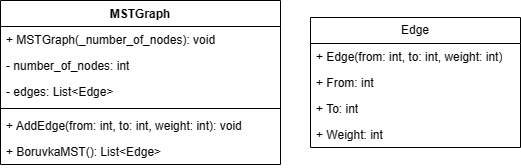
\includegraphics[width=0.8\textwidth]{class_diagram_boruvka_alg.png}
\end{figure}
\pagebreak

\subsection{Jarníkův algoritmus}
Algoritmus vybere první bod, pojmenujme si ho A. Nalezneme nejbližšší bod k A, pojmenujme ho B. Propojíme body a vznikne nám kostra A-B. Dále nalezneme nejbližší bod kostry A-B, pojmenujme ho bod C. Propojíme kostru A-B a bod C. Takto pokračujeme dokud nenalezneme minimální kostru grafu.
Algoritmus je tedy takzvaný greedy algoritmus.
Implementace vznikla v jazyce C\# dle následujícího pseudo-kódu.

\subsubsection{Psuedo-kód}
\begin{lstlisting}[language=csh]
    Založ prázdný seznam MST.
    Založ pole visited o délce počtu bodů.
    Nastav první bod jako navštívený.
    Zvyš počítadlo navštívených bodů na 1.

    Dokud je počet navštívených bodů nižší než celkový počet bodů
        Založ minEdge - nejlevnější cesta a nastav jí na null.
            Také by se dala použít nejvyšší hodnota v grafu.
        Pro každou cestu
            Pokud je začátek cesty navštívený a konec cesty nenavštívený
                Pokud je minEdge null NEBO cena vybrané cesty menší než cena minEdge
                    Nastav minEdge na vybranou cestu.
                Nebo pokud je navštívený konec cesty a začátek nenavštívený
                    Nastav minEdge na vybranou cestu.
            Pokud je minEdge null
                Hoď vyjímku - graf není propojený.
            Přidej minEdge do MST
            Pokud není začátek cesty navštívený
                Označ ho jako navštívený.
                Zvyš počet navštívených bodů o 1.
            Pokud není konec cesty navštívený
                Označ ho jako navštívený.
                Zvyš počet navštívených bodů o 1.
    Vrať MST.
\end{lstlisting}
\pagebreak
\subsubsection{C\#}
Jarníkův algoritmus využívá stejné podpůrné třídy, tedy Edge a MSTGraph jako Borůvkův algoritmus. Byly tedy vynechány. Soubor program.cs je také stejný, samozřejmě kromě volání Borůvkova algoritmu, místo toho voláme Jarníkův algoritmus.
\begin{lstlisting}[language=csh]
    public List<Edge> JarnikMST()
        {
            List<Edge> minimumSpanningTree = new List<Edge>();
            //Create an array to keep track of visited nodes
            bool[] visited = new bool[number_of_nodes];
            //Set the first node as visited
            visited[0] = true;
            int visited_count = 1;
            //Go through all nodes
            while (visited_count < number_of_nodes) {
                //Keep track of the edge with the lowest cost
                Edge? minEdge = null;
                //Find the cheapest edge
                foreach (Edge edge in edges) {
                    if (visited[edge.From] && !visited[edge.To]) {
                        if (minEdge == null || edge.Weight < minEdge.Weight) {
                            minEdge = edge;
                        }
                    }
                    else if (visited[edge.To] && !visited[edge.From]) {
                        if (minEdge == null || edge.Weight < minEdge.Weight) {
                            minEdge = edge;
                        }
                    }
                }
                //If a cheapest edge is not found the graph isn't connected
                if (minEdge == null) {
                    throw new Exception("Tree is not connected.");
                }
                //Add the cheapest edge to the MST
                minimumSpanningTree.Add(minEdge);
                //Set both origin and destination nodes as visited
                if (!visited[minEdge.From]) {
                    visited[minEdge.From] = true;
                    visited_count++;
                }
                if (!visited[minEdge.To]) {
                    visited[minEdge.To] = true;
                    visited_count++;
                }
            }

            return minimumSpanningTree;
        }
\end{lstlisting}
\pagebreak
\subsubsection{Class diagram}
\begin{figure}[h]
	\centering
	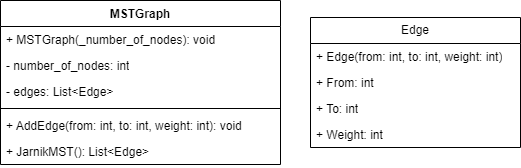
\includegraphics[width=0.8\textwidth]{class_diagram_jarnik_alg.png}
\end{figure}

\end{document}